%LTeX: language=de-DE
\chapter{Steckbrief}
    \section{Einordnung}
        Acrylnitril-Butadien-Styrol oder kurz ABS ist ein Terpolymer, dass zur Gruppe der (amorphen) Thermoplasten gehört. Aufgrund
        der chemischen Struktur ist eine weitere Unterordnung in die \enquote{hochschlagfesten Styrol-Copolymere} möglich \cite{Eyerer.2020.Polymer.Engineering.1}.

        Weitere bekannte Vertreter der amorphen Thermoplaste sind das Polyvinylchlorid (PVC), Polystyrol (PS), Polycarbonat (PC)
        oder Polymethylmethacrylat (PMMA). Ihnen allen gemein ist eine gute bis sehr gute optische Transmissivität bedingt durch ihren amorphen Aufbau (vgl. \cref{tab:steckbeef}).
        % \newpage
        \subsection{Varianten und Vergleich}
            Die folgenden Diagramme sollen einen Überblick über die wichtigsten Schlüsseleigenschaften des ABS im direkten Vergleich
            mit seinen Verwandten Derivaten und Polycarbonat als Referenz liefern. Werte wurden jeweils auf das in seiner
            Kategorie am besten abschneidende Material normiert und bilden damit relative Größen ab. Dies erschien sinnvoll,
            da es einen Vergleich \enquote{auf einen Blick} zulässt.

            \begin{figure}[h]
                \centering
                \includesvg[inkscapelatex=false, width=\textwidth]{RadarCharts/mechanical/mechanical.svg}
                \caption[Mechanisches Profil]{Mechanisches Profil.}
                \label{fig:pc mechanical profile}
            \end{figure}\par
            %
            \Cref{fig:pc mechanical profile} zeigt die mechanische Performanz des ABS\@. Neben anderen zur Auswahl stehenden
            Metriken wurde sich hier der Übersicht halber auf die Vergleichsgrößen Reißdehnung, Kugeldruckhärte, Biegefestigkeit
            und im Falle der Kunststoffe insbesondere dem Kriechmodul beschränkt.

            Es ist zu erkennen, dass ABS hier selbst im Vergleich zu seinen Derivaten unterwältigt. Einzig das
            Acrylnitril-Styrol-Acrylat (ASA) liegt hier in etwa gleichauf. Die thermischen und insbesondere die chemischen Profile
            (\cref{fig:pc thermal profile} und \cref{fig:pc chemical profile}) geben eine leicht differenzierteres Bild.

            Auch thermisch unterliegt überwiegend das ABS\@. Es zeigt sich, dass die Stärke des Materials in seinem chemischen
            Profil verortet zu sein scheint.

            Es sei an dieser Stelle angemerkt, dass ASA als eine Weiterentwicklung des ABS zu verstehen ist (siehe \cref{sec:geschichte}).
            So überrascht es wenig, dass dem gegenüber ABS in vielen Punkten unterliegt.
            % \newpage
            \begin{figure}[H]
                \centering
                \includesvg[inkscapelatex=false, width=\textwidth]{RadarCharts/thermal/thermal.svg}
                \caption[Thermisches Profil]{Thermisches Profil.}%
                \label{fig:pc thermal profile}
            \end{figure}
            %
            \begin{figure}[H]
                \centering
                \includesvg[inkscapelatex=false, width=\textwidth]{RadarCharts/chemical/chemical.svg}
                \caption[Chemisches Profil]{Chemisches Profil.}%
                \label{fig:pc chemical profile}
            \end{figure}
            \newpage
            \nocite{datenblattsammlung.KERN.20210201}
        \subsection{Preis}
            In Westeuropa wird ABS derzeit – unabhängig davon, ob es sich um regranuliertes oder \textit{virgin}\footnote{Dt.\ jungfräulich – Material zum Erstgebrauch.}
            ABS handelt – zwischen ca. €0,85 und €3,00 je Kilogramm gehandelt \cite{rohstoffboerse.kunststoffweb.de.20210206}.
            Als Rohstoff zur additiven Fertigung bewegen sich Preise – je nach Marktsegment – zwischen €15 und €120.

    \section{Herstellung}
        ABS besteht aus den drei Monomeren Acrylnitril, Butadien und Styrol. Die folgenden Abschnitte sollen einen groben
        Überblick zur Synthese der jeweiligen Monomere verschaffen, um darauf aufbauend Verfahren zur Polymerisation aufzuzeigen.
        
        \subsection*{Acrylnitril}
            Eine Möglichkeit der Synthese von Acrylnitril, die technisch heute noch in großem Maßstab umgesetzt wird, ist das nach dem gleichnamigen
            Unternehmen benannte \textsc{Sohio}-Verfahren (siehe \cref{sec:geschichte}).

            Die Ausgangsstoffe sind hier Propen, (Luft-)Sauerstoff und Ammoniak. In Gegenwart eines mineralischen Katalysators wird der Wasserstoff
            des einfach gebundenen Kohlenstoffatoms abgespalten und der Stickstoff des Ammoniaks lagert sich an. Die Edukte der
            stark exothermen Reaktion sind das gewünschte Acrylnitril und Wasser \cite{sohio.process.patent.1959.9201957}.

        \subsection*{Butadien}
            Das Monomer 1,3-Butadien findet in polymerisierter Form (Polybutadien) überwiegend in der Autoreifenindustrie als synthetischer Gummi
            Anwendung. Es ist ein Nebenprodukt bei der Aufspaltung langkettiger Kohlenwasserstoffe meist fossilen Ursprungs.

        \subsection*{Styrol}
            Eines der heute wichtigsten Verfahren zur Produktion von Styrol ist die Dehydrierung von Ethylbenzol
            an einem mineralischen Katalysator in Gegenwart von Wasserdampf unter hohem Druck \cite{styrol.synthese.Liquid.Phase.Alkylation.of.Benzene.Bellussi.1995}.

        \subsection{Polymerisation}
            Auf einem vorgelegten Polybutadienkautschuk werden Styrol und Acrylnitril aufgepfropft. Das so erhaltene Propfpolymerisat
            wird in der Regel mit einem SAN-Polymer versetzt, um das Endprodukt zu erhalten. Abstände und Verteilung der
            Propfkomponenten können eingestellt werden und beeinflussen Eigenschaften wie Härte, Fließverhalten oder
            Chemikalienbeständigkeit. Die Länge der dazwischenliegenden Polybutadienketten beeinflusst den Grad der Elastizität
            einerseits, die Anfälligkeit für Photooxidation andererseits \cite{Domininghaus.1998.Kunststoffe.und.ihre.Eigenschaften}.

            % Pfropfpolymerisation von Styrol und Acrylnitril auf einem vorgelegten Polybutadienlatex; das erhaltene Pfropfpolymerisat
            % wird mit einem getrennt hergestellten SAN-Latex abgemischt, koaguliert und getrocknet. \cite{Domininghaus.1998.Kunststoffe.und.ihre.Eigenschaften,Eyerer.2020.Polymer.Engineering.1}
    \section{Anwendung}\label{sec:anwendung}
            Aus der Kategorie der Kunststoffe ist Acrylnitril-Butadien-Styrol das meist verwendete Material für Produkt und
            Ingenieursanwendungen.
            Aufgrund seiner Temperaturbeständigkeit und hohen Schlagfestigkeit (vgl. hierzu \cref{fig:pc mechanical profile} und \cref{fig:pc thermal profile}) findet es breite Anwendung insbesondere in der
            Automobilindustrie zur Fertigung von Interieur, als Gehäuseteile für Elektronikprodukte oder auch Spielzeug. So verdankt etwa der Hersteller
            \textsc{LEGO} seinen Siegeszug der besonderen Eigenschaftenkomposition des Terpolymers. Die thermoplastische Komponente
            des in hohen Anteilen vorhandenen Polystyrols macht die Produktion einfach, schnell, günstig und damit geeignet
            für die Massenproduktion. Die durch das 1,3-Butadien verliehene Elastizität sorgt für Formbeständigkeit auch bei
            wiederholter Nutzung der \textsc{LEGO}-Steine.

            \begin{wrapfigure}{l}{.5\linewidth}
                \centering
                % \vspace{-\baselineskip}
                \adjustbox{max width=.5\textwidth}{
                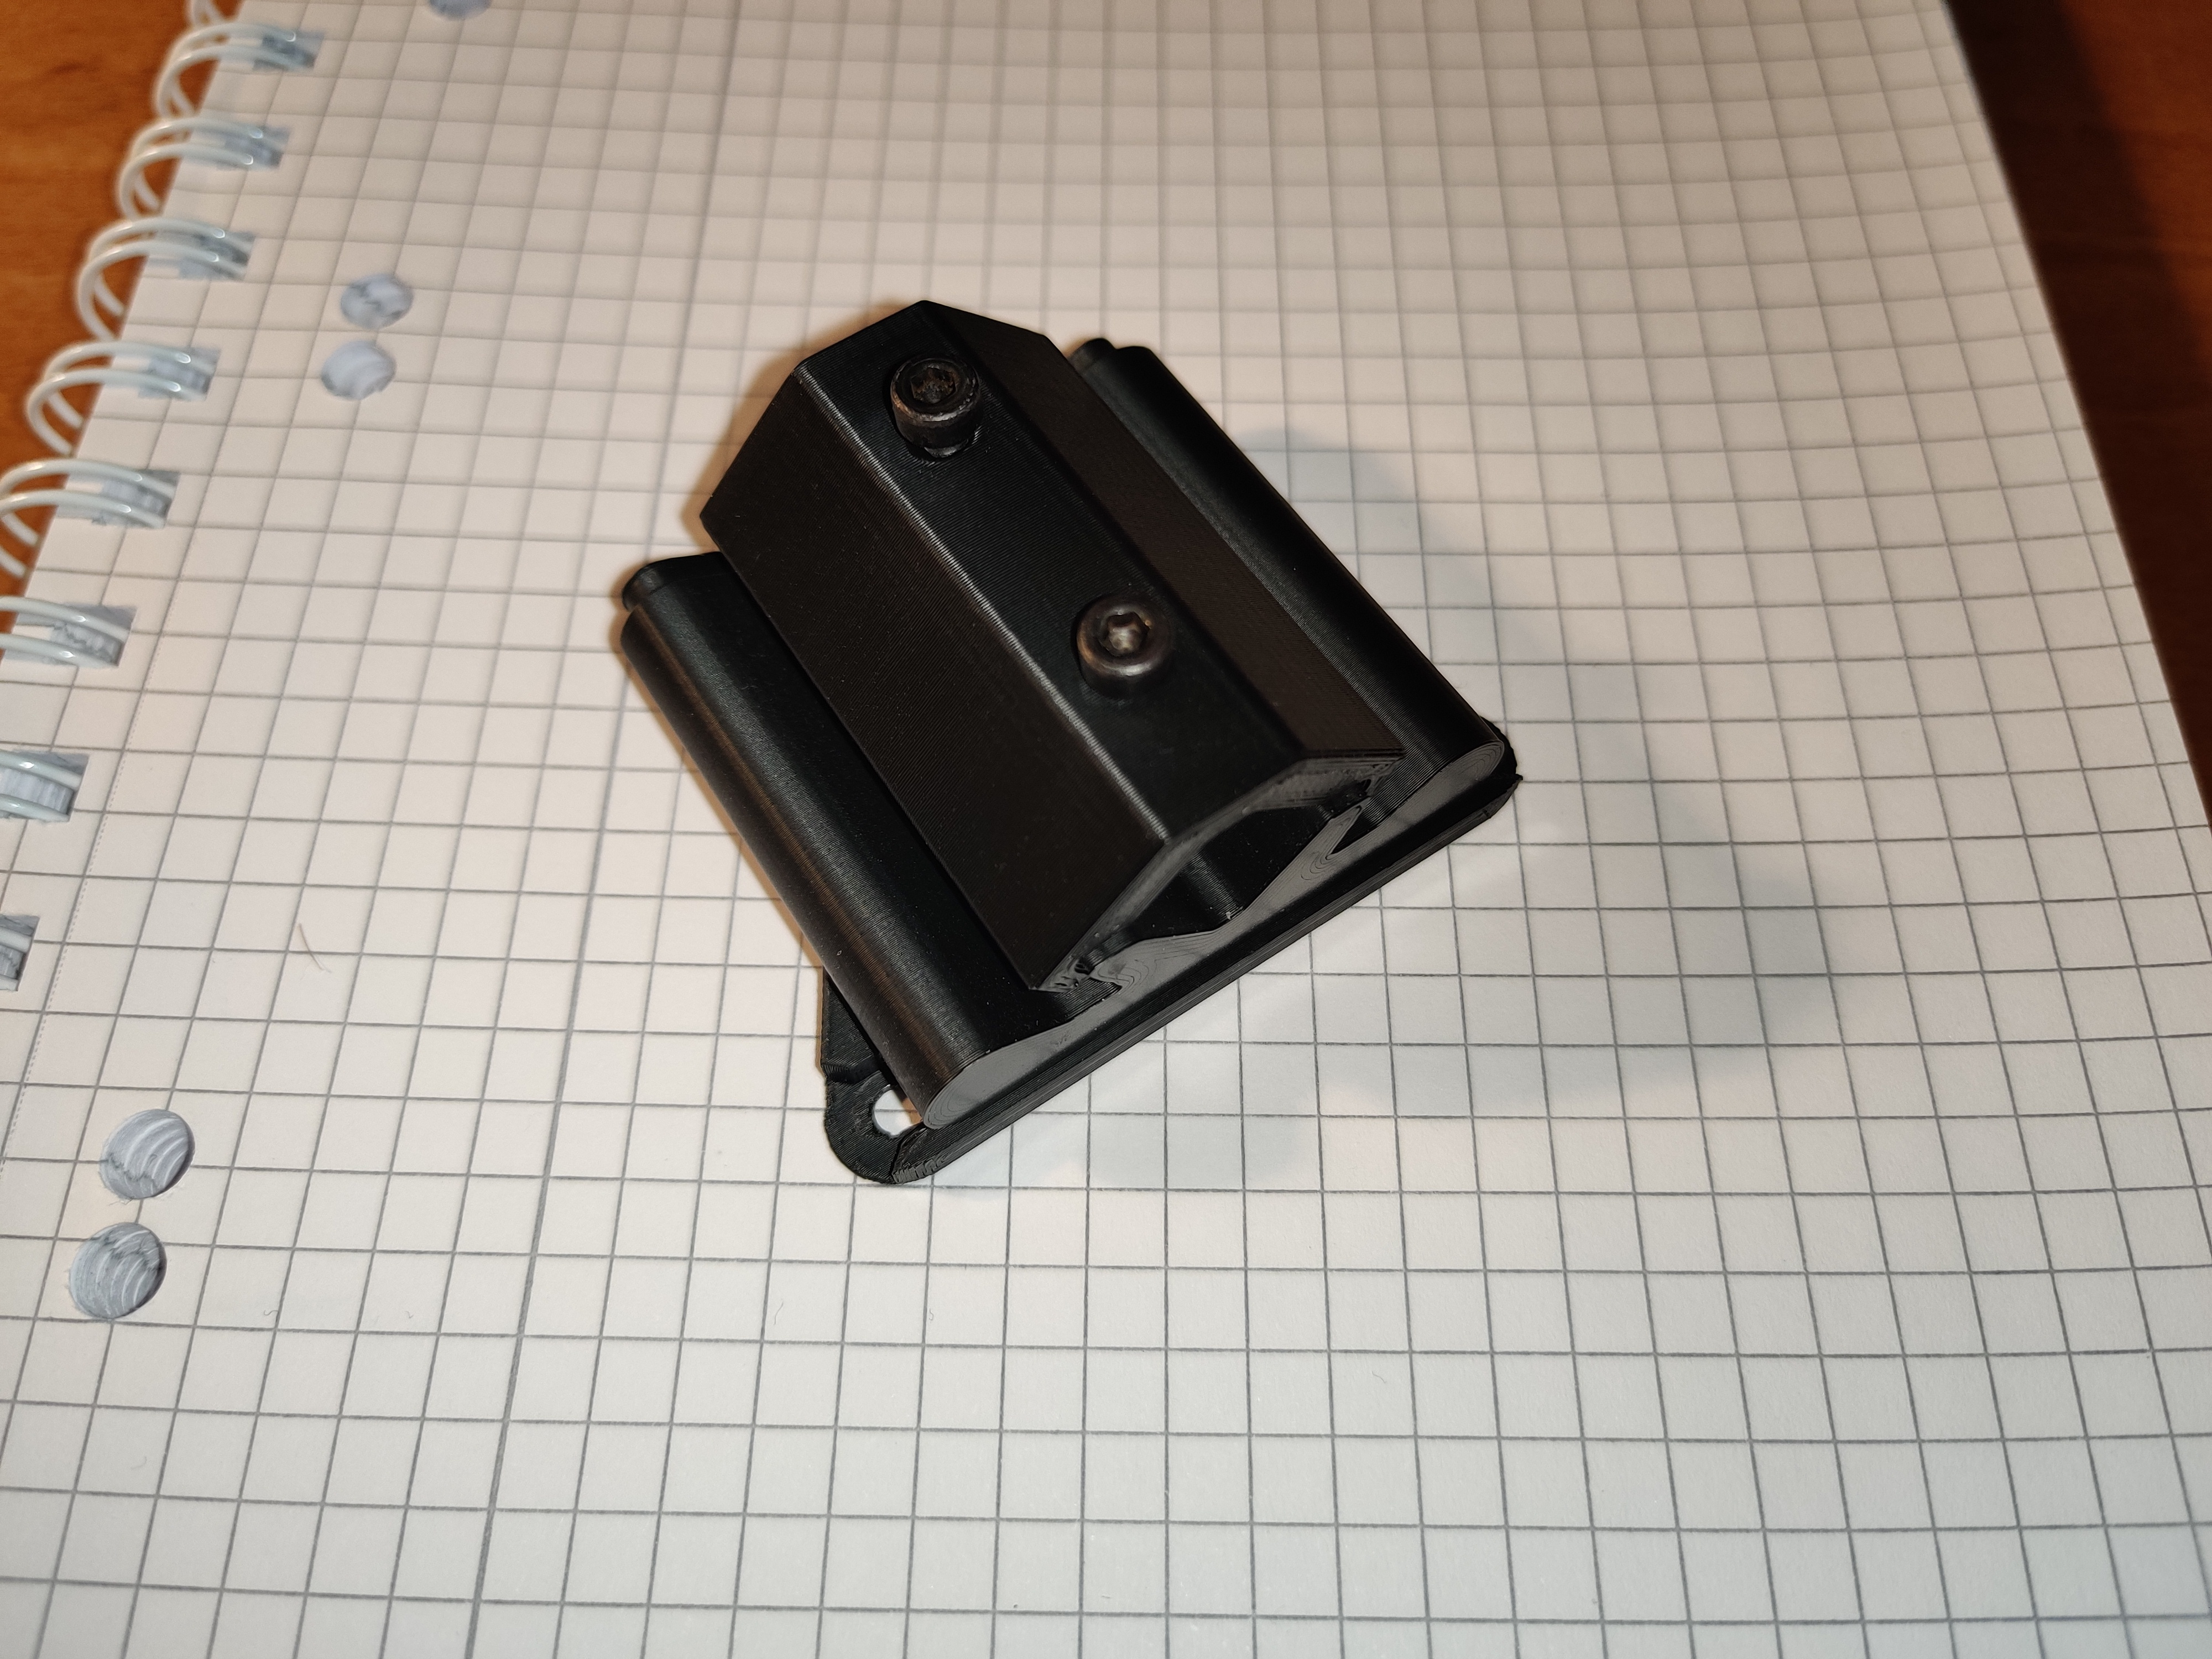
\includegraphics[width=\linewidth]{Assets/FDM_ABS/abs_teilA.jpg}
                }
                \caption[Eine aus schwarzem ABS im FDM-Verfahren gefertigte Stiftfixierung]{Eine aus schwarzem ABS im FDM-Verfahren gefertigte Stiftfixierung für einen Eigenbau-Stiftplotter.}%
                \label{fig:3dDruck ABS teil}
            \end{wrapfigure}
            Eine weitere, heute nicht mehr zu vernachlässigende Anwendung findet ABS als Rohmaterial in der additiven Fertigung
             – speziell im \textit{Fused Deposition Modeling}\footnote{Dt.: Schmelzschichtmodellierung.} – sowohl im Hobby-
            wie im professionellen Bereich. Hierbei wird das Material – zuvor zu einem Faden von üblicherweise \SI{1,75}{mm}
            Durchmesser extrudiert und aufgespult – innerhalb einer Düse bei Temperaturen zwischen \SI{240}{} und \SI{260}{\celsius} aufgeschmolzen
            und durch selbige Schicht um Schicht aufgetragen um das gewünschte Teil zu Formen. Seine in diesem Prozess gute
            Verarbeitbarkeit verdankt das Material seinen günstigen thermischen Eigenschaften, sowie seiner Eigenschaft in
            Aceton gut löslich zu sein. Dem Fertigungsverfahren intrinsisch weisen die fertigen Teile eine relativ hohe
            Oberflächenrauigkeit auf. Wenn gewünscht lassen sich die Teile mit handelsüblichem Aceton bedampfen, um so
            dem Druckguss vergleichbare Oberflächengüte zu erreichen. Nachteilhaft wirkt sich jedoch sein in diesem Anwendungsgebiet
            vergleichsweise hoher Längenausdehnungskoeffizient von \(\approx \SI{40-110}{\nicefrac{\micro m}{K}}\) (\cref{tab:steckbeef}) aus. Während des Verarbeitungsprozesses muss die umgebende Luft
            auf Temperaturen deutlich über Raumtemperatur gehalten werden während nennenswerte Schwankungen der Temperatur
            möglichst unterdrückt werden müssen, um unerwünschte Deformationen oder schlimmstenfalls einen vollständigen
            Verlust der Druckbetthaftung zu verhindern\footnote{\textit{Warping} oder zu Deutsch Verziehen/Verwölben.}.

    \section{Struktur und Eigenschaften}
            % \section{Strukturformel}
            \Cref{fig:strukturformeln_monomere} zeigt die Strukturformeln der beteiligten Monomere während in \cref{fig:strukturformeln polymere}
            die jeweiligen polymeren Formen dargestellt sind. Insbesondere in Blick auf den Butadienkautschuk ist erkennbar,
            dass nach der Polymerisation sich mittig eine kunjugierte Doppelbindung ausbildet flankiert von Einfachbindungen,
            die wiederum als Andockstellen für weitere Polymere dienen. Im Falle weiterer Butadienpolymere als Bindungspartner
            bilden sich alternierende Doppel- und Einfachbindungen. Letztere geben dem Endmaterial seine duktile Komponente und
            damit seine Schlagfestigkeit. So erschließt sich, dass die Duktilität des vorliegenden ABS mit der Länge
            dieser Butadienketten skaliert.\par
            Eine eher mäßige Wetterstandfestigkeit rührt von eben diesem Polybutadien-Rückrad her. Die Doppelbindung (erkennbar
            in \cref{subfig:structural formula polybutadiene}) des
            Butadiens wird durch einfallendes Licht im ultravioletten Spektralbereich angeregt. In Gegenwart von Sauerstoff
            werden Polymerketten unter Bildung von Hydroxyl- und Carboxylgruppen aufgespalten. Ultimativ führt dies zu
            (frühzeitiger) Alterung des Materials was sich wiederum als Verfärbung und Minderung der mechanischen Eigenschaften äußert.
            Um dem entgegenzuwirken werden mitunter zwar Fotostabilisatoren und/oder Radikalfänger eingesetzt, in der 
            Regel jedoch wird das ABS, um seine mechanischen Eigenschaften möglichst zu erhalten, mit einem schützenden Lack
            überzogen oder galvanisch behandelt \cite{Thermal.and.Photo-Degradation.of.Unstabilized.ABS.Adeniyi.1984,Domininghaus.1998.Kunststoffe.und.ihre.Eigenschaften}.
            \begin{figure}[H]%
                \centering
                \adjustbox{max width=.3\textwidth}{
                    \subfloat[Acrylnitril.\label{subfig:structural formula acrylonitril}]{\includesvg[inkscapelatex=false, scale=.65]{zeichnungen/acrylnitril.svg}}%
                }
                \qquad
                \adjustbox{max width=.3\textwidth}{
                    \subfloat[Styrol.\label{subfig:structural formula styrene}]{\includesvg[inkscapelatex=false, scale=.65]{zeichnungen/styrol.svg}}%
                }
                \qquad
                \adjustbox{max width=.3\textwidth}{
                    \subfloat[1,3-Butadien.\label{subfig:structural formula butadiene}]{\includesvg[inkscapelatex=false, scale=.65]{zeichnungen/butadien.svg}}%
                }
                \caption[Strukturformeln der monomeren Bestandteile des ABS]{Strukturformeln der monomeren Bestandteile des ABS.}%
                \label{fig:strukturformeln_monomere}%
            \end{figure}
            Unter anderem in Form von Nitrilhandschuhen ist das Copolymer aus Acrylnitril und
            1,3-Butadien unter der Bezeichnung Nitrilkautschuk gut bekannt. Der Butadienanteil verleiht dem Material seine Elastitzität,
            die stark polare Nitrilgruppe seine chemische Beständigkeit. Gleiches leistet das Polyacrylnitril in der Butadien-Styrol-Matrix.
            %
            \begin{figure}[H]%
                \centering
                \adjustbox{max width=.3\linewidth}{
                    \subfloat[Polyacrylnitril.\label{subfig:structural formula polyacrylonitril}]{\quad\includesvg[inkscapelatex=false, scale=.65]{zeichnungen/polyacrylnitril.svg}\qquad}%
                }
                \qquad
                \adjustbox{max width=.3\linewidth}{
                    \subfloat[Polystyrol.\label{subfig:structural formula polystyrene}]{\qquad\includesvg[inkscapelatex=false, scale=.65]{zeichnungen/polystyrol.svg}\qquad}%
                }
                \qquad
                \adjustbox{max width=.3\linewidth}{
                    \subfloat[Polybutadien.\label{subfig:structural formula polybutadiene}]{\qquad\includesvg[inkscapelatex=false, scale=.65]{zeichnungen/polybutadien.svg}\qquad}%
                }
                \caption[Strukturformeln der polymeren Bestandteile des ABS]{Strukturformeln der polymeren Bestandteile des ABS.}%
                \label{fig:strukturformeln polymere}%
            \end{figure}
            % Chemische und thermische Standfestigkeit durch Acrylnitril, Thermoplastisch verformbar durch Polystyrol, Zähigkeit
            % und Schlagfestigkeit durch 1,3-Butadien.
            
            Mischungsverhältnisse dieser drei Komponenten nach dem Schema \(\left[A_kB_lS_m\right]_n\) (vgl. \cref{fig:abs_struktur}) beeinflussen jeweils
            die mit ihnen assoziierten Eigenschaften des Gesamtmaterials. Hierdurch lassen sich durch relativ einfache Weise eine Großzahl verschiedener Varianten zum
            spezialisierten Einsatz produzieren. Dies spiegelt sich in der Vielzahl der auf dem Markt erhältlichen und unter
            verschiedenen Handelsnamen vertriebenen Varianten wider.
            \begin{figure}[H]
                \centering
                \adjustbox{max width=.39\linewidth}{
                \includesvg[]{zeichnungen/abs_struktur.svg}
                }
                \caption[Verallgemeinerte Darstellung der Makrostruktur des Polymers]{Eine verallgemeinerste Darstellung der Makrostruktur des ABS. Die Indices \(k,l,m\) geben
                die kontinuierlichen Anzahlen der jeweiligen Monomere und der Index \(n\) die Anzahl der aneinandergereihten Gesamtpolymerketten zum Makropolymer an.}
                \label{fig:abs_struktur}
            \end{figure}
    \section{Besonderheiten}
            Wie bereits in den vorherigen Kapiteln erwähnt, bietet ABS eine Mischung günstiger mechanischer Eigenschaften
            bei gleichzeitig hoher Oberflächengüte, Kratzfestigkeit und lässt sich darüber hinaus besonders gut oberflächenbehandeln
            ohne  Notwendigkeit von potenziell umwelt- oder gesundheitsschädlichen Zusatzstoffen. Sollen seine
            Eigenschaften auf einen bestimmten Anwendungszweck hin abgestimmt werden, kann dies durch bloßes Ändern der
            Mischverhältnisse seiner Bestandteile erfolgen. Das zusammen macht ABS zu einem breit anwendbaren Allround-Material.

            Weiterhin ist reines ABS für Lebensmittelkontakt zugelassen und erfüllt bei entsprechender Wahl der Füllstoffe
            Kriterien zu medizinischen Anwendung nach ISO 10993 \cite{ABS.M30i.Datasheet.Stratasys.20210210}.